\chapter{Introduction}\label{ch:introduction}
In the recent years we have been witnessing an incredible increase of
Artificial Intelligence (AI) applications and services.
Machine Learning (ML) and Deep Learning (DL) have been outperforming other
classical AI algorithms in many fields, like face recognition and natural
language processing.

This has been possible thanks to the explosion of data availability and compute
power, both needed and essential for ``training'' these neural networks.
Once the neural network has been trained, it can be used for the target that it
has been trained for: this phase is called ``inference''.
In \autoref{sec:training} I explain more in details these phases and what lies
in between.

Applications that requires some intelligence are computation intensive
demanding CPU, GPU, memory hence power out of the device and this makes the
application not always available to the end user.
In the last years the performance of these devices has been getting better and
better but still not sufficient for all more compute intensive applications.

The solution is to have a centralised data management and processing
(see~\ref{fig:centralised_intelligence}): the device collects data, send the
data to the cloud for processing and it receives back a response to their
request. This is called \textbf{centralised intelligence}.
Although this design is the basis of many applications, it presents some
drawbacks:
\begin{itemize}
    \item \textbf{amount of data}: the data generated by the device is sent to
        the cloud for processing. The amount of this data is not trivial and
        this could put under stress communication channels.
    \item \textbf{persistent connection}: in order to have a working
        application a persistent network connection between the device and the
        cloud computing is required.
    \item \textbf{real-time}: some applications cannot function properly when
        in presence of latency introduced by the communication between the
        device and cloud and any delay in processing the request by the cloud.
    \item \textbf{data privacy}: the device might send personal data to the
        cloud exposing privacy issues in case of hacking of leaking of
        information from the cloud provide.
\end{itemize}

\begin{figure}[ht]
    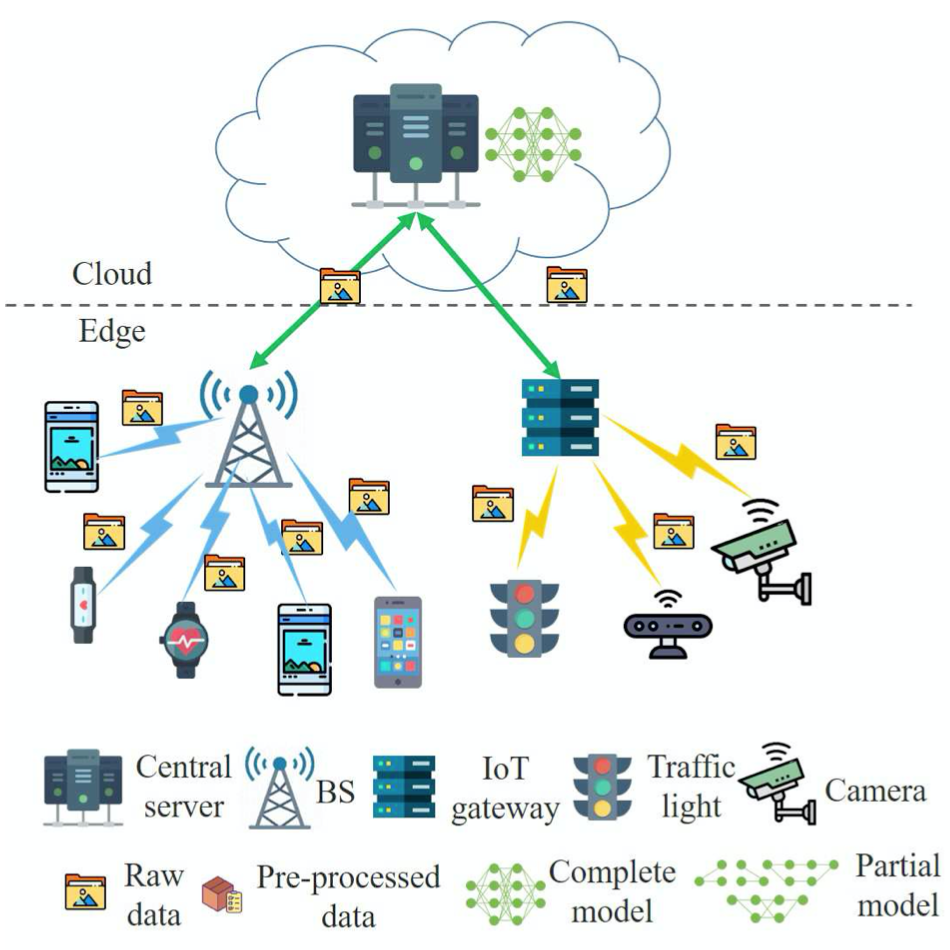
\includegraphics[width=10cm]{images/introduction/centralised_intelligence.png}
    \centering
    \caption{Centralised intelligence}\label{fig:centralised_intelligence}
\end{figure}

In order to overcome to the above issues, a different approach is needed where
the data processing is not centralised but distributed closer where it is
generated: this different approach is called \textbf{edge computing},
Computing, storage and networking resources are located at the edge of the
network (IoT gateways, routers, etc\ldots) whilst end devices like mobile
phones and IoT devices request services from edge servers are called edge
devices.
It is easy to understand how this approach can address some of the issues in
the centralised intelligence: low latency between edge devices and edge servers
and data exchange and data privacy are some how mitigated.
It is worth noticing that edge computing is not a replacement for cloud
computing. On the contrary, it complements cloud computing and both are
targeting different kind of applications.

If we push a little more the design, the basis of edge computing combined with
AI creates what is called
\textbf{edge or mobile intelligence} (see~\ref{fig:edge_intelligence}).

This means that the data collection, caching, processing and analysis happens
on the device where the data is generated.
With this model latency, data privacy, network load and communication are all
contained and improved, giving a better experience to the end user and making
the application more reliable.

\begin{figure}[ht]
    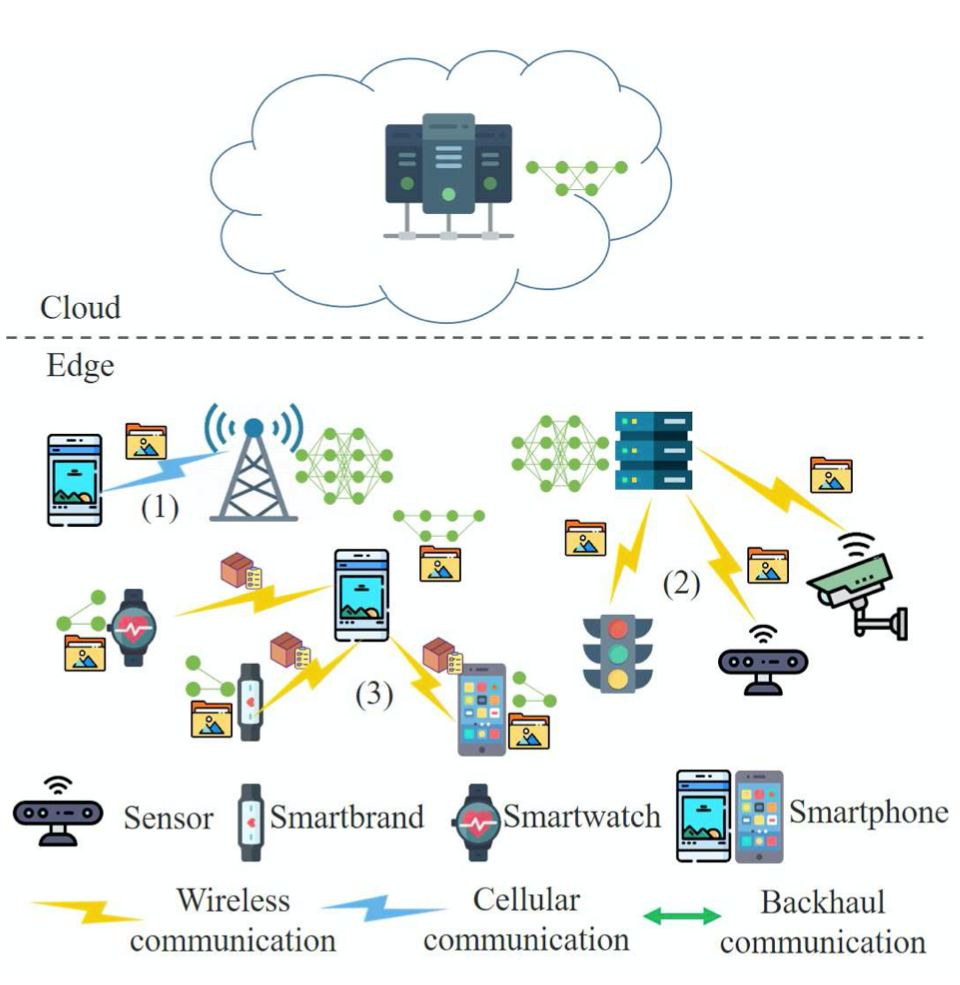
\includegraphics[width=10cm]{images/introduction/edge_intelligence.png}
    \centering
    \caption{Edge intelligence}\label{fig:edge_intelligence}
\end{figure}

With more powerful end devices we start having edge intelligence applications
in our pockets like smart suggestions on the keyboards based on the context of
the text, photos application with integrated face recognition (note: no
personal data is sent to the cloud) based on contacts stored on the mobile and
voice recognition commands for offline translation and on mobile actions.
Other examples are also self-driving cars, real-time applications and medical
devices but also noise cancellation on video call application like Microsoft
Teams. Interestingly enough, as counter example Google Meet uses its model on
the cloud leveraging Google TPU infrastructure.

In this thesis I focus mainly on the \textbf{edge inference} (~\ref{fig:edge_inference})
and specifically how the models can be optimised in order to reduce memory
footprint, size and compression without losing any accuracy in the prediction.

\begin{figure}[ht]
    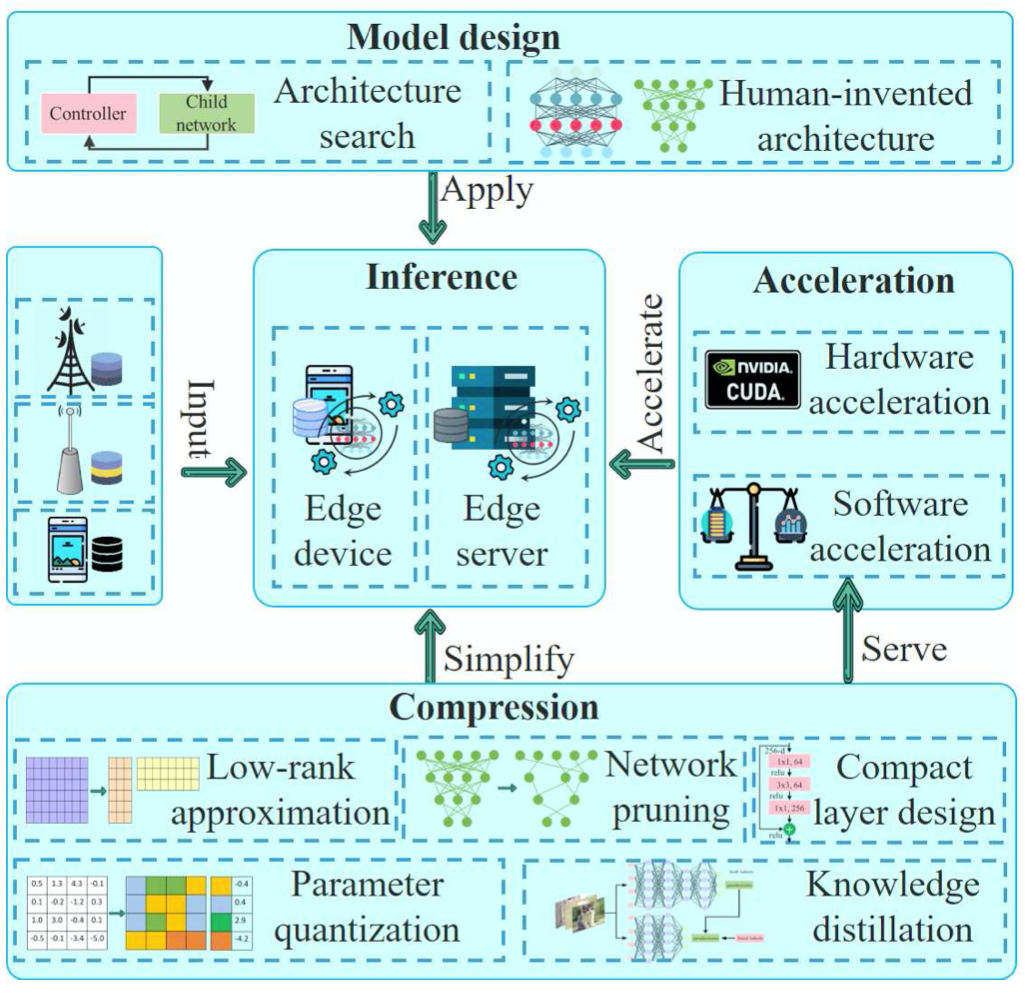
\includegraphics[width=10cm]{images/introduction/edge_inference.png}
    \centering
    \caption{Edge inference}\label{fig:edge_inference}
\end{figure}

Edge inference is the final step of a model life cycle where the trained model
is used to infer new and unseen data via a forward pass of the neural network.
This step happens on the edge device and it presents some challenges due to the
limited amount of compute power and memory on the device itself.

In order to work correctly end efficiently the model needs to go through a
series of optimisations that decreases the power/memory consumption and latency
whilst maintaining the accuracy at acceptable levels \- ideally without
incurring in any decrease.

As the figure~\ref{fig:edge_inference} shows, there are different techniques
that it can be used to optimise models for edge inference. These are:
\begin{itemize}
    \item \textbf{Model design}: let the machines themselves design optimal
        models or human-invented architectures
    \item \textbf{Acceleration}: hardware acceleration mainly focus on parallel
        execution while software acceleration focuses on optimising resource
        management and compilers, based on compressed models
    \item \textbf{Compression}: low-rank approximation, knowledge distillation,
        compact layer design, network pruning and parameters quantization are
        few techniques in order to achieve model compression
\end{itemize}

The above introduction~\cite{xu2020edge} sets the background for this thesis where
I focus on a specific technique of model pruning.
In \autoref{sec:training} I give an overview of the entire flow of an
intelligence application giving a brief explanation of every step of the flow.

In \autoref{sec:MO} I explain the main techniques for model optimisation for
deployment, explaining what they are, pros and cons.

In \autoref{ch:pruning} I show the pruning technique more in details and
the section \autoref{sec:heuristic} illustrate the theory behind the per-layer
pruning configuration with heuristic.

In \autoref{ch:implementation} I show the code I have implemented in
TensorFlow Model Optimisation giving full explanation and some working
examples.

Finally in \autoref{ch:results} I report experiment results on few well known
neural networks showing the benefits of this approach.

Unless specified otherwise, \textbf{all the examples, code and documentation
assume the use of TensorFlow (\url{https://www.tensorflow.org/}) and its
ecosystem.}

\section{From training to inference}\label{sec:training}

The pillars of edge intelligence are \textbf{data, model and computation}.
We need big amount of data in order to train a model that behaves as expected.
Computation is needed throughout the whole process, from training to edge
inference.

\begin{figure}[ht]
    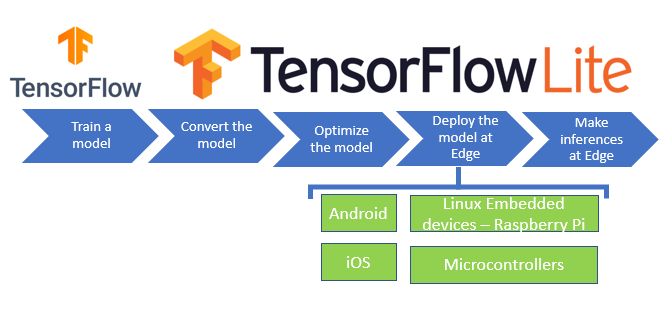
\includegraphics[width=10cm]{images/introduction/training_inference_flow.png}
    \centering
    \caption{From training to edge inference}\label{fig:training_inference}
\end{figure}

The figure \autoref{fig:training_inference} shows a classic life cycle flow of
an intelligent application. A brief explanation of each step:

\begin{itemize}
    \item \textbf{Train a model}: once decided what the task is, the right
        model needs to be used. There are different options: create a custom
        model, use a pre-trained model or use Transfer Learning on a
        pre-trained model.
    \item \textbf{Convert the model}: once the model is trained, it needs to be
        converted in a special format (\texttt{.tflite}) that can be used on
        edge devices in efficient manner.
    \item \textbf{Optimise the model}: that's the key phase where the model is
        optimised to use less space/memory and to have a faster inference by
        decreasing the latency. More details will be presented in section
        \autoref{sec:MO}.
    \item \textbf{Deploy the model at Edge}: once the model has been optimised,
        it is ready to be deployed to the edge device.
    \item \textbf{Make inference at Edge}: this is the last step where finally
        the model is used to do inference on new data that it has never seen
        and hopefully giving expected results in a timely fashion.
\end{itemize}

The above flow shows the big picture of an intelligent application life
cycle~\cite{tflite:intro} and gives an idea of the complexity behind the
creation of an edge intelligent application.
In the rest of the chapter, I will explain what techniques are available in
TensorFlow in order to \textbf{optimise the model}.

\section{Model optimisations for deployment}\label{sec:MO}

To optimise TensorFlow models, the ecosystem offers \textit{TensorFlow Model
Optimisation Toolkit} (abbrev. \textit{TFMOT}) which minimizes the complexity
of optimising machine learning inference.

Inference efficiency is a critical concern when deploying machine learning
models because of latency, memory utilization, and in many cases power
consumption. Particularly on edge devices, such as mobile and Internet of
Things (IoT), resources are further constrained, and model size and efficiency
of computation become a major concern.

Computational demand for training grows with the number of models trained on
different architectures, whereas the computational demand for inference grows
in proportion to the number of users.

Model optimisation is useful, among other things, for:

\begin{itemize}
    \item Reducing latency and cost for inference for both cloud and edge
        devices (e.g.\ mobile, IoT).
    \item Deploying models on edge devices with restrictions on processing,
        memory and/or power-consumption.
    \item Reducing payload size for over-the-air model updates.
    \item Enabling execution on hardware restricted-to or optimised-for
        fixed-point operations.
    \item Optimising models for special purpose hardware accelerators.
\end{itemize}

The available techniques are:

\begin{itemize}
    \item \textbf{Weight Clustering}: Clustered models are those where the
        original model's parameters are replaced with a smaller number of
        unique values.
    \item \textbf{Quantization}: Quantized models are those where we represent
        the models with lower precision, such as 8-bit integers as opposed to
        32-bit float. Lower precision is a requirement to leverage certain
        hardware.
    \item \textbf{Weight Pruning}: Sparse models are those where connections in
        between operators (i.e.\ neural network layers) have been pruned,
        introducing zeros to the parameter tensors.
\end{itemize}

When pre-optimised models and post-training tools do not satisfy your use case,
the next step is to try the different training-time tools.

Training time tools piggyback on the model's loss function over the training
data such that the model can ``adapt'' to the changes brought by the
optimisation technique.~\cite{tfmot:intro}

\subsection{Weight clustering}
Clustering, or weight sharing, reduces the number of unique weight values in a
model, leading to benefits for deployment. It first groups the weights of each
layer into N clusters, then shares the cluster's centroid value for all the
weights belonging to the cluster.

\begin{figure}[ht]
    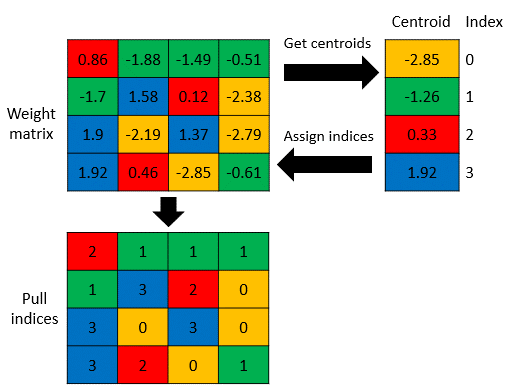
\includegraphics[width=\textwidth]{images/introduction/weight_clustering.png}
    \centering
    \caption{Weight clustering}\label{fig:weight_clustering}
\end{figure}

A brief explanation of \autoref{fig:weight_clustering}. For example a layer in
the model contains a 4$\times$4 matrix of weights (represented by the
``weight matrix'' in \autoref{fig:weight_clustering}). Each weight is stored
using a float32 value. When the model is saved, 16 unique float32 values are
stored to disk.

Weight clustering reduces the size of the model by replacing similar weights in
a layer with the same value. These values are found by running a clustering
algorithm over the model’s trained weights. The user can specify the number of
clusters (in this case, 4). This step is shown in ``Get centroids'' in the
diagram, and the 4 centroid values are shown in the ``Centroid'' table. Each
centroid value has an index (0\-3).

Next, each weight in the weight matrix is replaced with its centroid’s index.
This step is shown in ``Assign indices''. Now, instead of storing the original
weight matrix, the weight clustering algorithm can store the modified matrix
shown in ``Pull indices'' (containing the index of the centroid values), and
the centroid values themselves.

In this case, the size has been reduced from 16 unique floats, to 4 floats and
16 2-bit indices. The savings increase with larger matrix sizes.

Note that even if we still stored 16 floats, they now have just 4 distinct
values. Common compression tools (like zip) can now take advantage of the
redundancy in the data to achieve higher compression.

Weight clustering has an immediate advantage in reducing model storage and
transfer size across serialization formats, as a model with shared parameters
has a much higher compression rate than one without. This is similar to a
sparse (pruned) model, except that the compression benefit is achieved through
reducing the number of unique weights, while pruning achieves it through
setting weights below a certain threshold to zero. Once a model is clustered,
the benefit of the reduced size is available by passing it through any common
compression tool.

To further unlock the improvements in memory usage and speed at inference time
associated with clustering, specialized run-time or compiler software and
dedicated machine learning hardware is required.~\cite{tfmot:clustering_blog}

This technique brings improvements via model compression. Future framework
support can unlock memory footprint improvements that can make a crucial
difference for deploying deep learning models on embedded systems with limited
resources.

According to Google experiments, models can be compressed up to 5x with minimal
loss of accuracy. Here below results on
vision~\autoref{fig:clustering_image_classification} and speech
models~\autoref{fig:clustering_keyword_spotting}.

\begin{figure}[ht]
    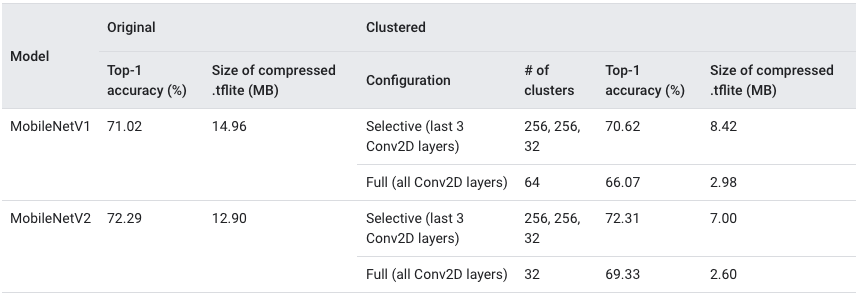
\includegraphics[width=\textwidth]{images/introduction/clustering_image_classification.png}
    \centering
    \caption{Weight clustering on image classification}\label{fig:clustering_image_classification}
\end{figure}


\begin{figure}[ht]
    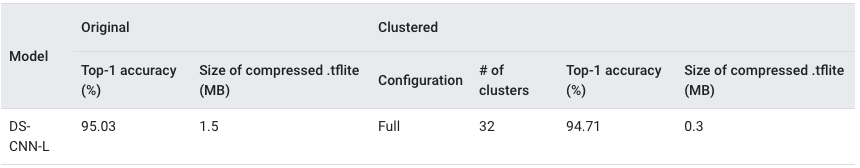
\includegraphics[width=\textwidth]{images/introduction/clustering_keyword_spotting.png}
    \centering
    \caption{Weight clustering on keyword spotting}\label{fig:clustering_keyword_spotting}
\end{figure}

Size of compressed \texttt{.tflite} refers to the size of the zipped
\texttt{.tflite} file obtained from the model from the following process:

\begin{enumerate}
    \item Serialize the Keras model into \texttt{.h5} file
    \item Convert the \texttt{.h5} file into \texttt{.tflite}
    \item Compress the \texttt{.tflite} file into a zip
\end{enumerate}

The weight clustering implementation is based on the \textit{Deep Compression:
Compressing Deep Neural Networks With Pruning, Trained Quantization and Huffman
Coding}~\cite{han2015deep}~\cite{tfmot:clustering}

\subsection{Quantization}
There are two forms of quantization: \textbf{post-training quantization} and
\textbf{quantization aware training (QAT)}. The former is easy to use whilst
the latter often offers better model accuracy.

\subsubsection{Quantization is lossy}
Quantization is the process of transforming an ML model into an equivalent
representation that uses parameters and computations at a lower precision.
This improves the model's execution performance and efficiency

However, the process of going from higher to lower precision is lossy in
nature. As seen in \autoref{fig:quantization}, quantization squeezes a small
range of floating-point values into a fixed number of information buckets.

\begin{figure}[ht]
    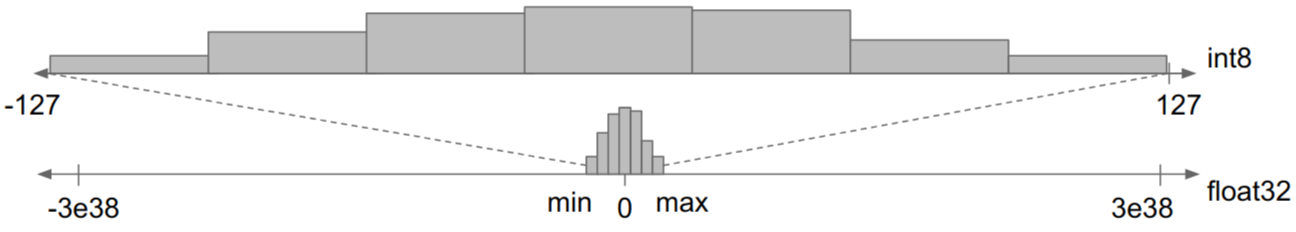
\includegraphics[width=\textwidth]{images/introduction/quantization.png}
    \centering
    \caption{Quantization}\label{fig:quantization}
\end{figure}

This leads to information loss. The parameters (or weights) of a model can now
only take a small set of values and the minute differences between them are
lost. For example, all values in range [2.0, 2.3] may now be represented in one
single bucket. This is similar to rounding errors when fractional values are
represented as integers.

There are also other sources of loss. When these lossy numbers are used in
several multiply-add computations, these losses accumulate. Further, int8
values, which accumulate into int32 integers, need to be rescaled back to int8
values for the next computation, thus introducing more computational
error.~\cite{tfmot:quantization_blog}

\subsubsection{Quantization aware training}
Quantization aware training emulates inference-time quantization, creating a
model that downstream tools will use to produce actually quantized models. The
quantized models use lower-precision (e.g. 8-bit instead of 32-bit float),
leading to benefits during deployment.

Quantization brings improvements via model compression and latency reduction.
With default API, Google has observed that the model shrinks by 4x and 1.5 \-
4x improvements in CPU latency. Eventually, latency improvements can be seen on
compatible machine learning accelerators (e.g.: EdgeTPU and NNAPI).

At the time of writing, QAT is still under development and has some limitations
regarding to its functionality (distributed training, limited support for
Subclassed Models, RNN/LSTM models, stable APIs, etc\ldots)

\begin{figure}[ht]
    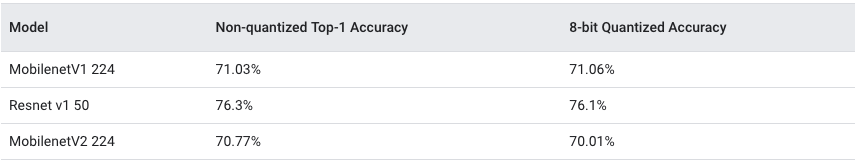
\includegraphics[width=\textwidth]{images/introduction/qat_image_classification.png}
    \centering
    \caption{QAT on image classification}\label{fig:qat_image_classification}
\end{figure}

The models in \autoref{fig:qat_image_classification} were tested on ImageNet
and evaluated in both TensorFlow and TFLite.

For background on something similar, see the \textit{Quantization and Training
of Neural Networks for Efficient Integer-Arithmetic-Only Inference}
paper~\cite{Jacob_2018}.
This paper introduces some concepts that this tool uses.
The implementation is not exactly the same, and there are additional concepts
used in this tool (e.g.\ per-axis quantization).~\cite{tfmot:quantization_training}

\subsubsection{Post-training Quantization}
Post-training quantization includes general techniques to reduce CPU and
hardware accelerator latency, processing, power, and model size with little
degradation in model accuracy. These techniques can be performed on an
already-trained float TensorFlow model and applied during TensorFlow Lite
conversion. These techniques are enabled as options in the TensorFlow Lite
converter.

Two types of post-quantization exist:
\begin{itemize}
    \item \textbf{Quantizing weights}: Weights can be converted to types with
        reduced precision, such as 16 bit floats or 8 bit integers. Google
        generally recommends 16-bit floats for GPU acceleration and 8-bit
        integer for CPU execution. At inference, the most critically intensive
        parts are computed with 8 bits instead of floating point.
    \item \textbf{Full integer quantization of weights and activations}:
        Improve latency, processing, and power usage, and get access to
        integer-only hardware accelerators by making sure both weights and
        activations are quantized.  This requires a small representative data
        set. The resulting model will still take float input and output for
        convenience.
\end{itemize}

There are several post-training quantization options to choose from.
\autoref{fig:post_quantization_techniques} shows a summary table of the choices
and the benefits they provide.~\cite{tfmot:quantization_post_training}

\begin{figure}[ht]
    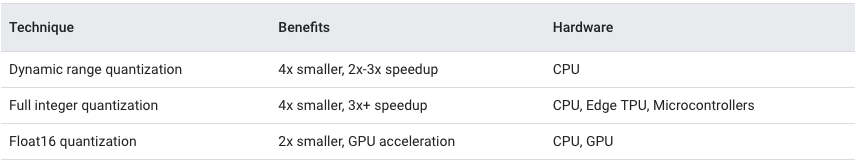
\includegraphics[width=\textwidth]{images/introduction/post_quantization_techniques.png}
    \centering
    \caption{Post-quantization techniques}\label{fig:post_quantization_techniques}
\end{figure}

Compared to their float counterparts, quantized models are up to 2–4x faster on
CPU and 4x smaller (See \autoref{fig:post_quantization_latency}).

\begin{figure}[ht]
    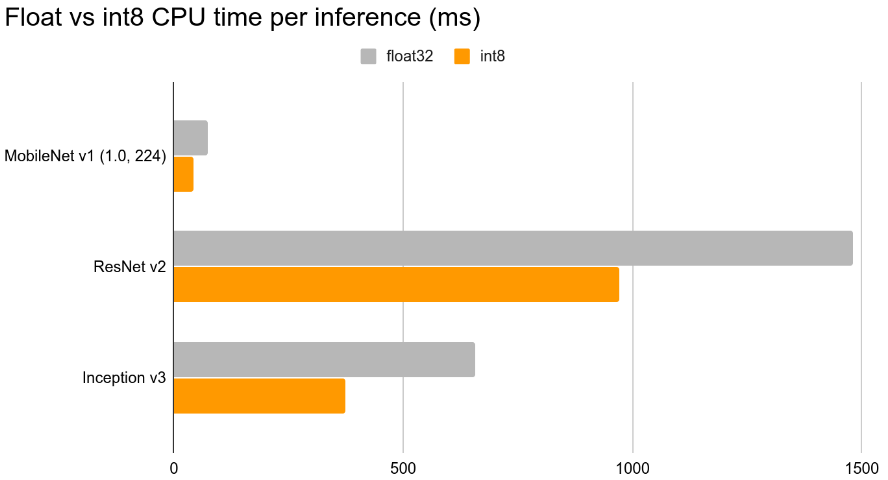
\includegraphics[width=\textwidth]{images/introduction/post_quantization_latency.png}
    \centering
    \caption{Post-quantization latency}\label{fig:post_quantization_latency}
\end{figure}

With just 100 calibration images from ImageNet dataset, fully quantized integer
models have comparable accuracy with their float versions (MobileNet v1 loses
1\%) (See \autoref{fig:post_quantization_accuracy}).

\begin{figure}[ht]
    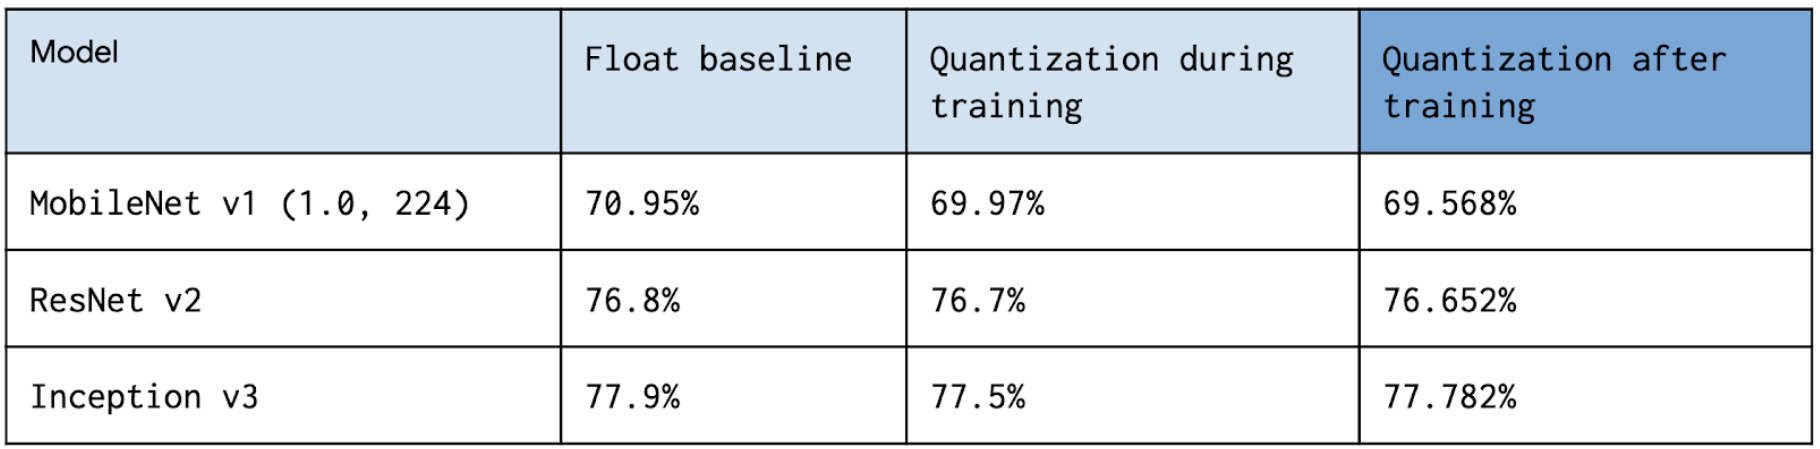
\includegraphics[width=\textwidth]{images/introduction/post_quantization_accuracy.png}
    \centering
    \caption{Post-quantization accuracy}\label{fig:post_quantization_accuracy}
\end{figure}

\subsection{Weight pruning}
Magnitude-based weight pruning gradually zeroes out model weights during the
training process to achieve model sparsity. Sparse models are easier to
compress, and we can skip the zeroes during inference for latency improvements.

This technique brings improvements via model compression. In the future,
framework support for this technique will provide latency improvements.
Google has seen up to 6x improvements in model compression with minimal loss of
accuracy.

The technique is being evaluated in various speech applications, such as speech
recognition and text-to-speech, and has been experimented on across various
visioni (see \autoref{fig:pruning_image_classification}) and translation
models (see \autoref{fig:pruning_translation}).~\cite{tfmot:pruning}

\begin{figure}[ht]
    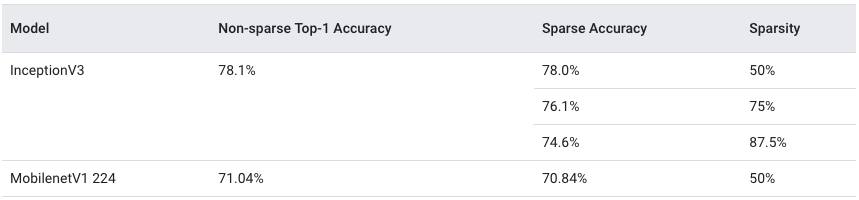
\includegraphics[width=\textwidth]{images/introduction/pruning_image_classification.png}
    \centering
    \caption{Weight pruning on image classification}\label{fig:pruning_image_classification}
\end{figure}

\begin{figure}[ht]
    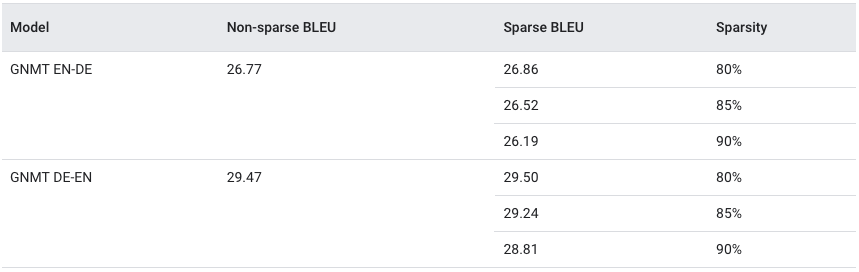
\includegraphics[width=\textwidth]{images/introduction/pruning_translation.png}
    \centering
    \caption{Weight pruning on translation}\label{fig:pruning_translation}
\end{figure}

In \autoref{ch:pruning} I will go more in details of this technique.

\subsection{Combine multiple optimisations}
The optimisation techniques shown in \autoref{sec:MO} bring excellent results
in terms of model size and latency.
The model can be optimised further combining those techniques. For instance the
model can be optimised using pruning, post-training quantization and then
compress the result with any compression algorithm (e.g.\ zip, gzip)
Similarly the model can be optimised using clustering, post-training
quantization and compression.
The optimisation can be pushed further including all the previous techniques as
shown in \autoref{fig:collaborative_optimisation}:

\begin{figure}[ht]
    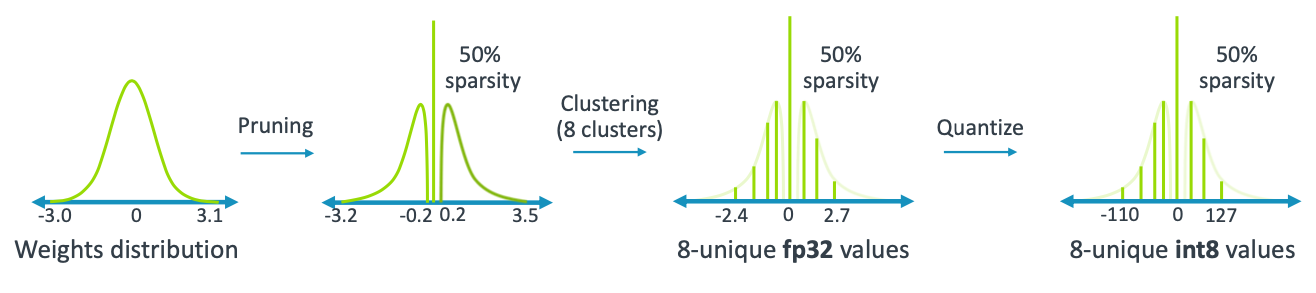
\includegraphics[width=\textwidth]{images/introduction/collaborative_optimisation.png}
    \centering
    \caption{Collaborative optimisation}\label{fig:collaborative_optimisation}
\end{figure}

\begin{enumerate}
    \item \textbf{Weight Pruning}: remove all near-zero weights
    \item \textbf{Weight Clustering}: group all the remaining weights in
        different clusters
    \item \textbf{Quantization}: the weights representing the clusters are
        quantized from floating point at 32 bit to integer at 16/8bit
    \item \textbf{Compression}: the last step is to apply a compression
        algorithm to the model in order to improve deployment
\end{enumerate}

The paper \textit{Deep Compression: Compressing Deep Neural Networks With
Pruning, Trained Quantization and Huffman Coding}~\cite{han2015deep} shows an
optimisation pipeline (See \autoref{fig:combine_multiple_optimisations})

\begin{figure}[ht]
    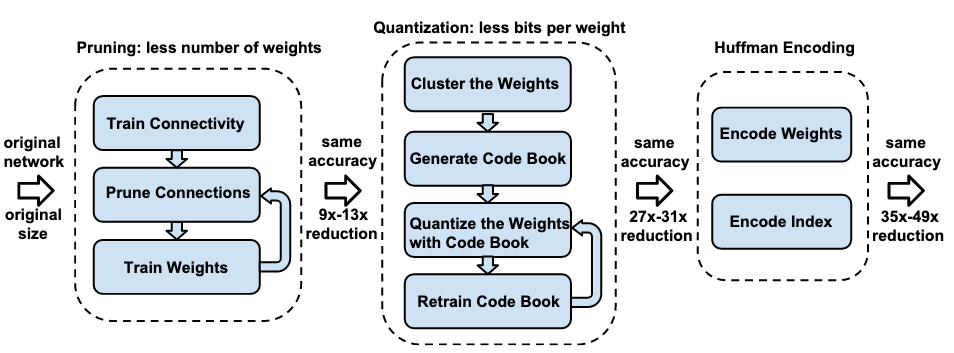
\includegraphics[width=\textwidth]{images/introduction/combine_multiple_optimisations.png}
    \centering
    \caption{Combine multiple optimisations}\label{fig:combine_multiple_optimisations}
\end{figure}

\autoref{fig:combine_multiple_optimisations} shows the three stage compression
pipeline: pruning, quantization (with clustering) and Huffman coding. Pruning
reduces the number of weights by 10×, while quantization/clustering further
improves the compression rate: between 27× and 31×. Huffman coding gives more
compression: between 35× and 49×. The compression rate already included the
meta-data for sparse representation. The compression scheme doesn't incur any
accuracy loss.
